\subsection{Problem Definition}

For my project, I will be creating a game, playable on a computer, that will allow people with limited time to still be able to enjoy playing a fun and engaging game. To begin with, I will list the current problems with games that are still playable.

\begin{enumerate}[label=\textbf{\arabic*.}]
    \item \textbf{Games have very long rounds} - This causes people to be involved in the same game for a much longer period of time, and results in there being time to only play one or two rounds at most, and potentially having to leave mid-way through a round if another tasks needs to be taken care of. This can result in frustration, especially if the person had favourable conditions, and may lead to them leaving the game entirely. 
    \item \textbf{Queue times for games are becoming very long} - This usually accompanies games which have long round times as the people who are playing are most likely in a game already, and so therefore, there are very few people left that can form a lobby. This also occurs whenever there is strict matchmaking rules, such as based on MMR, or region. This causes there to be a smaller pool of players that can be in the same lobby, and therefore, it is much more difficult to create a lobby in a short period of time.
    \item \textbf{Overly complicated} - Modern games are starting to have lots of additional features, due to the large amount of computing power that is available, and whilst this does mean that there are lots of things to experiment with in the game, it can make it overwhelming at times, and very competitive. This will suit some people, but for casual players, having a game with lots of different details can be very difficult to learn, and so discourages them from playing.
    \item \textbf{Cosmetic items} - Whilst these do add aesthetic appeal to the game, in most games they are locked behind a paywall, whilst leaving players who do not wish to spend money on a game feeling left out.
    \item \textbf{Intensive Hardware Requirements} - As the average PC has become more powerful, older devices can no longer keep up with modern games, and this means that lots of people are simply unable to play with people who have a modern PC. This is mostly due to the large maps and intensive graphics, that require lots of CPU and GPU processing power. Most games do have options to reduce the graphics quality, but they still require newer hardware to be able to play. Someone who is not in a position to purchase a newer device will then be excluded from playing.
    \item \textbf{Too strategy based} - An issue within the shooter genre which I aim to fix is that games are becoming very strategy based instead of focusing on fast-paced intense gameplay. This is done by reducing the player's movement speed and by making maps very intricately designed. However, this can make it boring at times, because players spend a lot of time hiding in spots, or setting up traps instead of fighting with other players. This also leads to the sensation that the game is boring, leading people to not want to play anymore.
    \item \textbf{Too competitive} - Many games have a match-making rating (MMR for short), which changes depending on whether you won or lost the game. This causes people to feel pressured during the game, and this can cause them to not enjoy playing, especially if they are casual players.
    \item \textbf{Lack of competent bots} - Many bots in games lack any proficiency in the game, and this means that they are not able to be put in a game if there are not enough players, or if someone leaves the game. This also means that if someone wants to train certain mechanics in the game, they do not have any quick way of checking. "Training" modes in most games are very empty, and usually consist of empty maps, or stationary targets that cannot retaliate.
\end{enumerate}

Based on this, I wanted to see how these factors impacted people's enjoyment of shooter games, and what my project should focus on in order to make the game more accessible and enjoyable to a wider range of people.

\subsection{Analysis of Existing Solutions}

Next, I will look at some other games that are available currently, and what their positive and negative aspects are, as well as what things I can learn from them and implement into my project.


\vs

\subsubsection{Chess}

Chess is a classic board game that is enjoyed by many people globally and has been around for centuries, and has been on the internet since the early 2000s. It involves moving pieces on a board according to a set of rules, and the player who loses is the one who no longer has any legal moves remaining. Recently, chess websites have seen a boom in popularity. Despite this, there are many people who don't enjoy or understand chess, and many that do. \cite{chess}
\begin{figure}[h!t]

\begin{annotatedFigure}
	{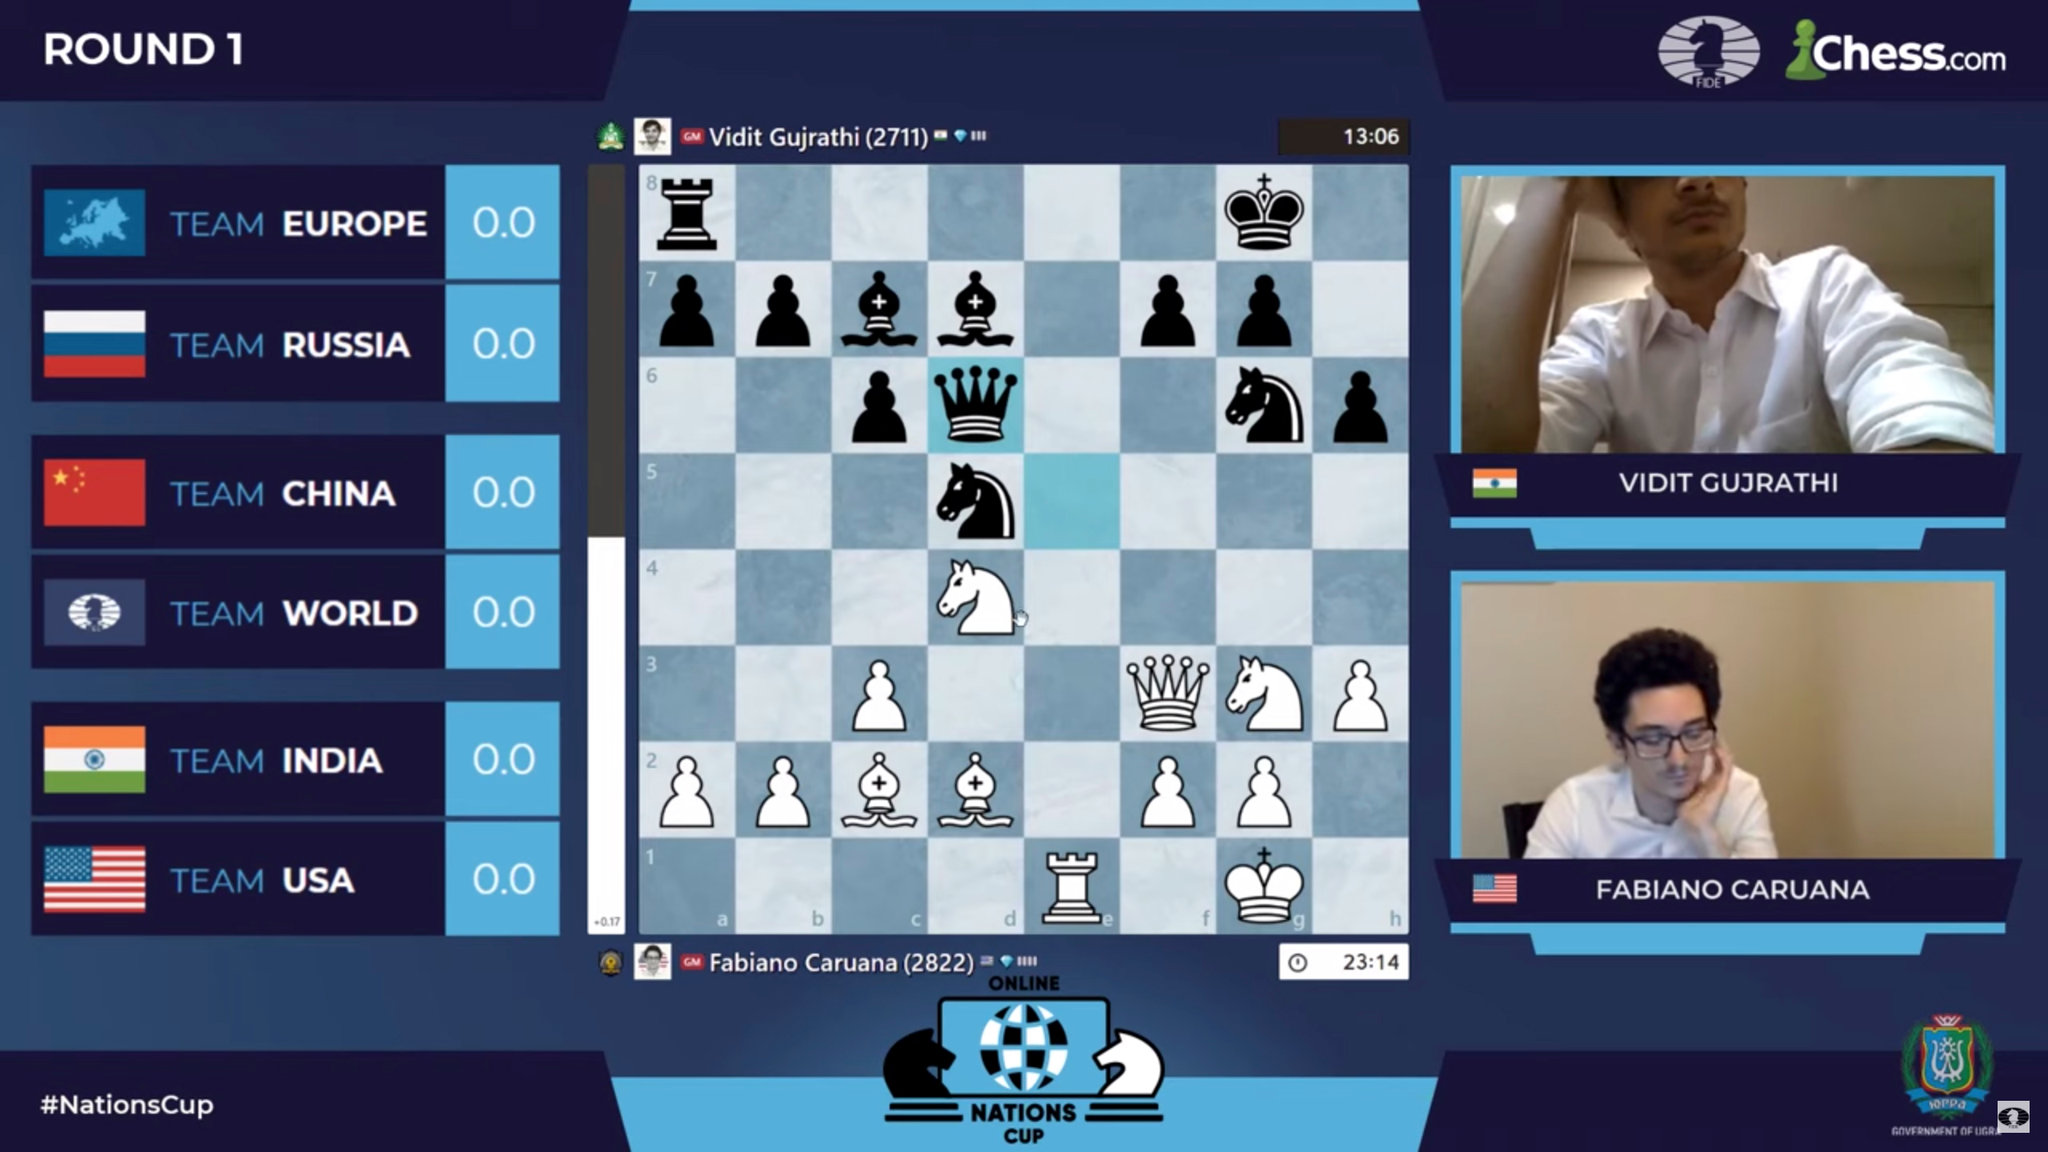
\includegraphics[width=1.0\linewidth]{Analysis/Images/ChessScreenshot.jpg}}
	\annotatedFigureBox{0.617,0.854}{0.696,0.9092}{A}{0.617,0.854}%bl
	\annotatedFigureBox{0.28,0.1773}{0.313,0.8736}{B}{0.28,0.1773}%bl
	\annotatedFigureBox{0.303,0.8416}{0.493,0.9305}{C}{0.303,0.8416}%bl
	\annotatedFigureBox{0.5,0.18}{0.693,0.2253}{D}{0.5,0.18}%bl
\end{annotatedFigure}
\caption{\textbf{Chess} - An image of a live stream of a professional chess tournament from }
\label{fig:chess_tournament}
\end{figure}

\textcolor{cyan}{\textbf{Analysis:}}
In box A, we can see the time left for each player in the game. This is important, since chess is usually played with a clock, and so it is useful to have this visible clearly to both players, but not in such a way that is intrusive on the player's vision of the board. Placing this near the corner of the board means that a player can easily how much time they or the opponent has left, but not be distracted by the clock.

\vs
In box B, we can see the computer analysis of the game. Normally, this would not be present during a rated game, but during live streams or analysis of games, it is put there to provide more information to players. Generally, chess positions are very complex, and therefore, it may not be obvious to inexperienced players what is going on, and so this is quite a useful tool. For players who are learning the game, it can be helpful to see where they may have blundered, and what moves would be better in that position.

\vs
In box C, we display the name and the rating of the player. This tells you who you are playing against and what their ELO is, which is a ranking often used in chess. This isn't particularly relevant, but it shows you that you are playing against a real player, which is a concern for some people. Additionally, if you want to play against friends, it's useful to make sure that you are playing against the right person. Another advantage is that it shows you if you are matched with a novice player or someone who has played the game for a long time, which may not affect the actions of the player directly, but it will inform them as to the level of play they can expect in the game.

\vs
Finally, the lettering on the bottom in Box D and the left edge of the board lets us easily identify which square a certain piece is on, and this is helpful when communicating with other players about moves, and is the standard notation for chess globally. This is useful, for example, for a coach who might want to help their play spot a move on the board.
\vs


\textcolor{green}{\textbf{Positives:}}
Chess is another game that satisfies my criteria and has another benefit. Online chess also lets people choose what length of game they want to play, ranging anywhere from 15 seconds to an hour. This is useful as it allows people to dedicate as much time as they want and no more than that for certain. It also has a ranking system, and is relatively easy to pick up. It is a reliable platform, and has been used for professional tournaments, such as during the pandemic, as seen in Figure \ref{fig:chess_tournament}. 
\vs


\textcolor{red}{\textbf{Negatives:}} Again, it's not an shooter game and not everyone likes or enjoys playing it. It isn't as visually stimulating as other games and for some people that is a major issue. In recent times, throughout the pandemic, chess gained a lot of popularity and many streamers became very popular and chess websites like \emph{chess.com} were not able to keep up with the demand, reaching 2 million players per day at one point. Another issue is that there is a very steep learning curve, and so the game can feel unrewarding when initially starting out, and requires a very large time investment to get good at the game. This is not always a possibility, and so people may feel unmotivated to play as it takes so long to understand how to becomes better at the game.
\vs


\textcolor{violet}{\textbf{Ideas taken:}} There are different time controls, which can be desirable so people can play as many rounds as they want depending on how much time they have, which would be ideal in my project, as time is a major restriction for most people. Additionally, the website \emph{chess.com} has bots on it that you can play against to practice with.
\vs


\subsubsection{Unreal Tournament}

Unreal Tournament is a series of games made by Epic Games starting in 1999 and the final game due to be released in 2017, but being cancelled before it was ever released. This final iteration was released in pre-alpha, but of course was not a final product. There is still some footage from the pre-alpha, so we will analyse that here.
\vs
\begin{figure}[h!t]
\begin{annotatedFigure}
	{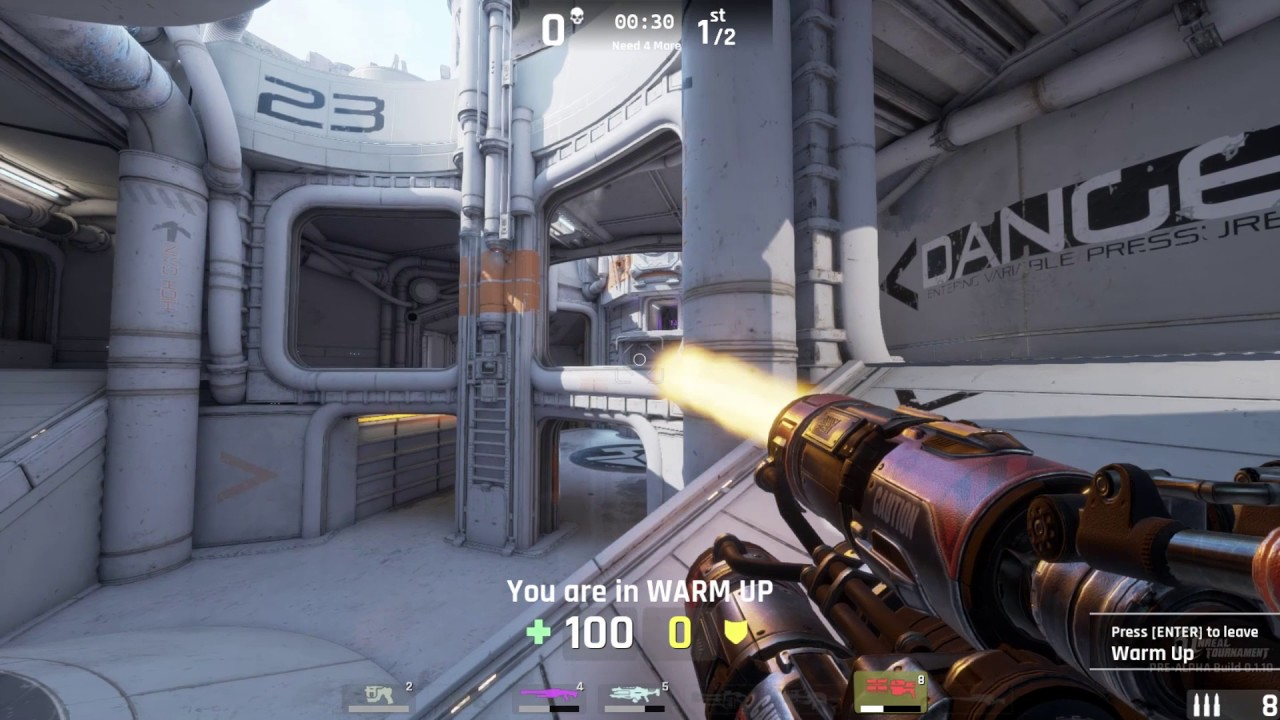
\includegraphics[width=1.0\linewidth]{Analysis/Images/UnrealTournament.jpg}}
	\annotatedFigureBox{0.4052,0.9022}{0.5982,0.9984}{E}{0.4052,0.9022}%bl
	\annotatedFigureBox{0.393,0.0891}{0.5972,0.1703}{F}{0.393,0.1703}%tl
	\annotatedFigureBox{0.842,0.0603}{0.9982,0.1593}{G}{0.842,0.0603}%bl
	\annotatedFigureBox{0.2580,0.000}{0.7380,0.0831}{H}{0.2580,0.0831}%tl
\end{annotatedFigure}
\caption{\textbf{Unreal Tournament} - Screenshot taken during gameplay from \cite{ut}}
\label{fig:ut}
\end{figure}

\textcolor{cyan}{\textbf{Analysis:}}
Starting in Box E, we can see that we gain important information about the game here in a concise way. We find what we need to do to win the game, how long is left in the game, and what position we are in the game. This is important for a player to know as it may advise them on how to proceed. For example, if there is a large amount to be done in order to win the game, the player knows to play more aggressively. This justifies it being there, because it informs the player's decisions during the game.

\vs
In box F, we see the player's health and shield levels. This is important information, since if the player is low health, they may choose to heal instead of engaging in combat, and vice versa. The information presented on the screen is in a large font which makes it easy to see the information at a glance, but not so big as to distract from the main information on the screen (ie. the game itself).

\vs
In Box H, we can see the player's weapons as well as how much ammo each one has. This allows a player to see what they have currently selected, and we can also see that on the screen. This is justified because having this information present allows a player to make an informed decision on what they should do next. For example, if they are on low ammo on all of their weapons, they should reload, or look for more ammo. It also tells them what types of strategies may work in the game, since different weapons have different characteristics which are more favourable in certain scenarios. For example, a sniper rifle might be more useful in a long-range encounter, but a shotgun might work better in close quarters. Having this information is useful to a player, and without it, they would struggle, and so it's justified to be there. It's isn't the most important piece of information however, so it doesn't occupy too much of the screen, and is at the bottom.

\vs
Finally, in Box G, we see the option to leave the warm up and to join the actual game. This is useful because it gives the player control over what they want to do, and it tells them what mode they are in currently. This is justified because new players may be confused about what they are doing if they haven't played before, or have been told what each mode is. Therefore, having a label describing what they are currently doing is incredibly helpful to them.
\vs


\textcolor{green}{\textbf{Positives:}} \emph{Unreal Tournament} is also a shooter game. The shortest game length is 4 minutes according to Wikipedia whereas I hope to make that 6 minutes, but in 3 separate rounds. The advantage of this is to make it so that people are able to dedicate less time to a specific round, so even if they lose, they still have a share of the time to win the round. 
\vs


\textcolor{red}{\textbf{Negatives:}} It is primarily a single-player game, which many people can find boring, and not as interactive as a multi-player game.An issue with Unreal Tournament is that and no servers are currently running, and so it results in people not being able to play it at all. This means that there are very few games similar to Unreal Tournament that are still available.
\vs


\textcolor{violet}{\textbf{Ideas taken:}} There are lots of different mechanics within the game such as those seen in \href{https://www.youtube.com/watch?v=knSzJbkofek}{this video}. These are inspirations for what can be implemented in my game, and what other things can be included in order to make it more dynamic.
\vs


\subsubsection{Valorant}

\emph{Valorant} is a highly successful First Person Shooter Game made by Riot Games.

\begin{figure}[h!t]

\begin{annotatedFigure}
	{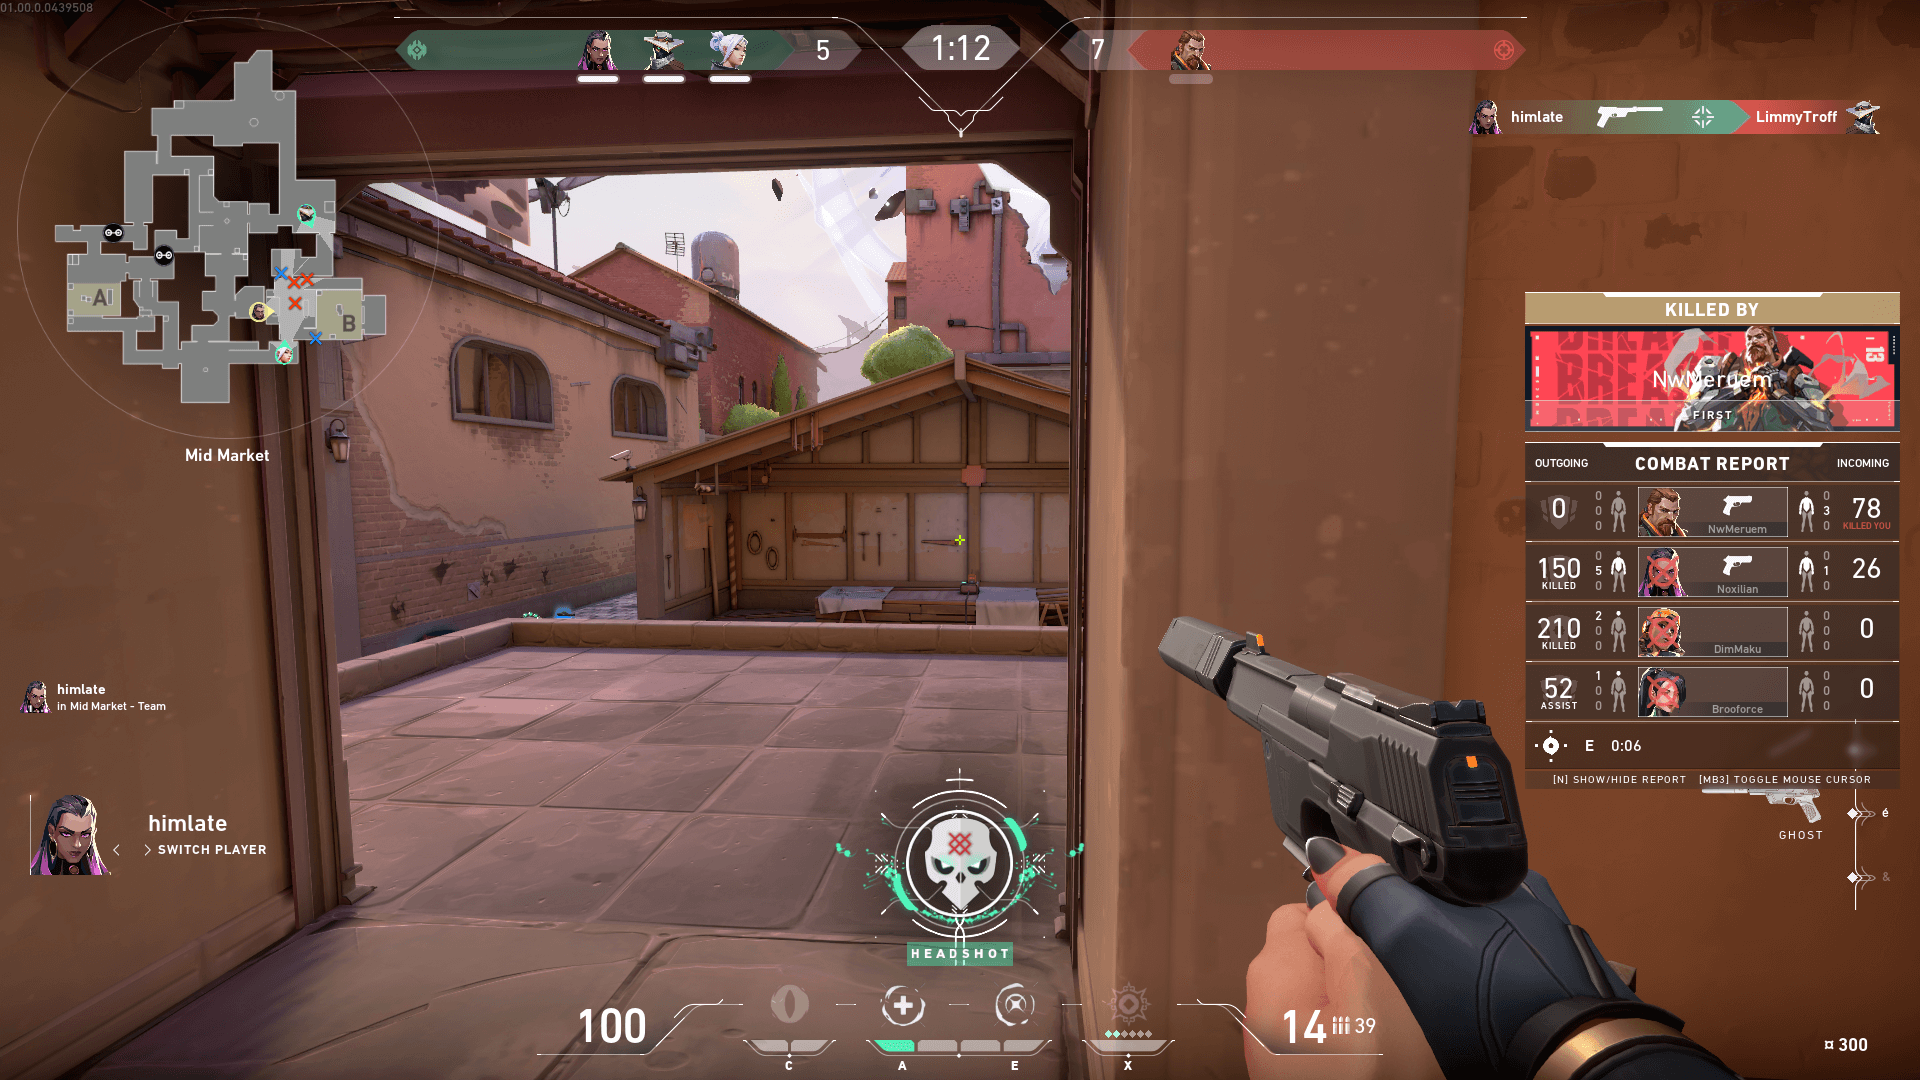
\includegraphics[width=1.0\linewidth]{Analysis/Images/ValorantScreenshot.png}}
	\annotatedFigureBox{0.189,0.9106}{0.8052,0.9949}{I}{0.189,0.9106}%bl
	\annotatedFigureBox{0.0252,0.6109}{0.2132,0.9639}{J}{0.0252,0.6109}%bl
	\annotatedFigureBox{0.757,0.848}{0.9862,0.938}{K}{0.757,0.848}%bl
	\annotatedFigureBox{0.215,0}{0.7762,0.1009}{L}{0.215,0.1009}%tl
\end{annotatedFigure}

\caption{\textbf{Valorant} - Screenshot of gameplay from \cite{val}}
\label{fig:valorant}

\end{figure}

\vs
%Screenshot Credit: https://interfaceingame.com/screenshots/valorant-headshot/

\textcolor{cyan}{\textbf{Analysis:}}
In box I, we see the players remaining in each team, the time left in the round, and the score. This is helpful because it informs all players of how they should play, and what strategies are most likely to get them a win in each round. For example, if one team has more players than another at some point in a round (due to some players being eliminated), they know that they can quite easily get a win.

\vs
In box J, we see a mini-map. This is quite a common feature amongst shooter games, and it allows players to see where they are, where their team-mates are, and where objectives are. This allows players to see the quickest way to get to their desired position. For new players, who may not know the layout and structure of the maps, it provides an intuitive way of understanding where they are relative to other players, as well as which direction they are facing. This is not made too large as too distract the player, but not too small so that the player cannot accurately see what is happening. Furthermore, the map is placed in the top left corner, because this allows the player to have a clear view of the middle row of their screen, which is where most of the action happens.

\vs
In box K, we see the elimination feed. This tells everyone in the game who has just been eliminated that round, which tells teams important information that informs their decisions. For similar reasons to the ones mentioned above, it is also placed in a corner, as it isn't the most important information the player is receiving.

\vs
At the bottom of the screen, we have box L. It shows the player the health that they have on the left hand side, the abilities in the middle, and the ammo left on the right hand side. The weapons that they have is on the right hand side of the screen, but was obscured in the image due to a popup from the game. The screen shown is from the view of a player who was eliminated earlier that round and is currently spectating one of their teammates. This is a useful feature because it means that a player is not just waiting around between rounds if they are eliminated, and can still be involved in the thrill of the game. From the viewpoint of a player who is still playing the middle of the right hand side of the screen would show the selection of weapons available to the player to use, and which button to press to select it. Icons are used to represent each weapon, because they each have distinctive shapes which are easy to identify. This is essential, because First Person Shooters are quite fast-paced with split-second decisions needing to be made, and so therefore, having a quickly recognisable symbol is crucial.


\vs
\textcolor{green}{\textbf{Positives:}} \emph{Valorant} is also a very successful game that is a shooter game. It also uses vibrant colours and interesting map design, combined with a wide range of abilities depending on the character taken. This allows for a lot of different situations to arise and means that the games are always varied and exciting. The UI is slightly larger than it is for other games, but it is still kept minimal and only conveys essential information. There is also a voice chat feature which allows players on the same team to talk to each other in real time during the game.

\vs
\textcolor{red}{\textbf{Negatives:}} The rounds are extremely long, even lasting over 45 minutes. This is a major problem for people who are on limited time, as they are much less likely to start a new game as they don't want to have to leave mid-way. This leads to people abandoning the game altogether, and subsequently not being able to play even if they do have a little bit of time.

\vs
\textcolor{violet}{\textbf{Ideas Taken:}} It has a very high skill ceiling (the maximum skill that a player can reach in the game) due to a large number of mechanics and different characters, which all specialise in different skills. This keeps the game interesting and unique. This is something that I am to replicate in my project by using movement mechanics, which allow a player to move very fast in a short period of time, and potentially "out-play" opponents. This adds to the intensity of the game, and also means that despite the short rounds people will see a lot of action in the games.
\vs

\subsubsection{Rocket League}

\emph{Rocket League} is a game made by Psyonix, and is played by millions. It involves scoring goals, using cars which can be driven around the map and even on the walls. The cars have boost which allows them to drive at extremely high speeds, but needs to be recharged as there is only a limited amount of it. This can be done by driving over pads or cylinders on the field which refills the boost by different amounts. The game has a very simple premise, but there are many mechanics within the game, which can be chained together to make complex motions, keeping the game interesting.


\begin{figure}[h!t]

\begin{annotatedFigure}
	{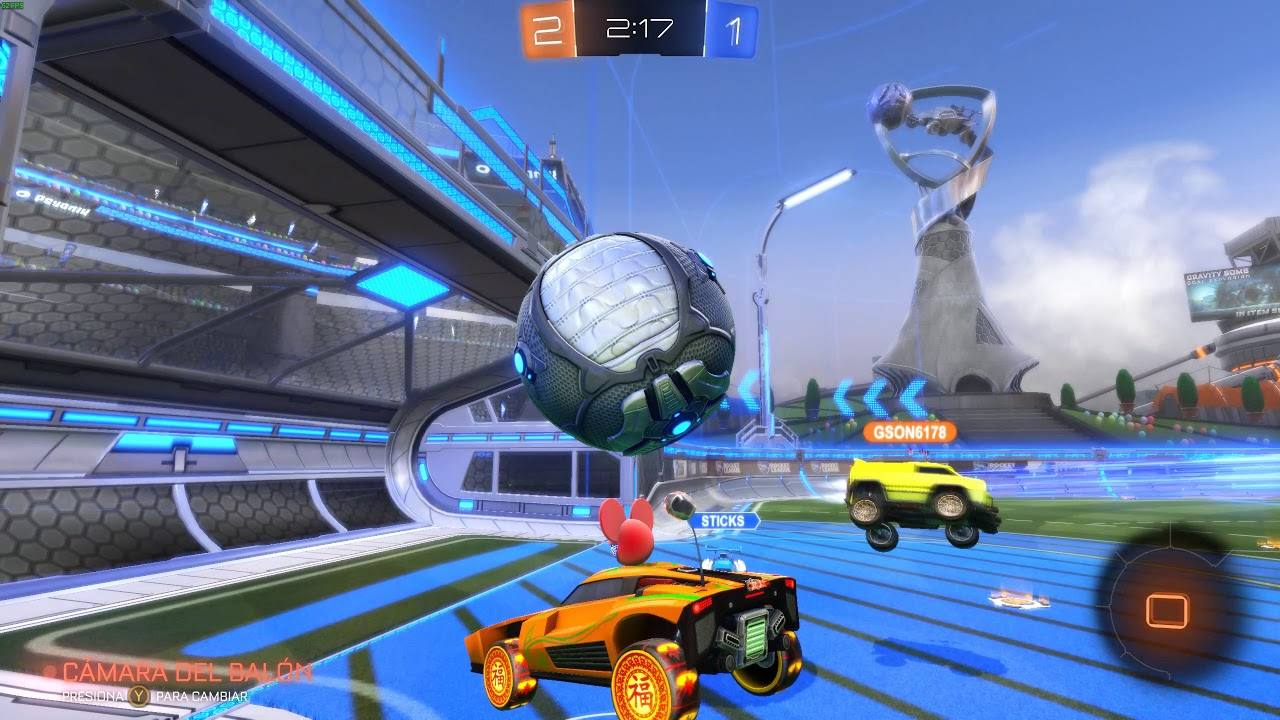
\includegraphics[width=1.0\linewidth]{Analysis/Images/RocketLeague.jpg}}
	\annotatedFigureBox{0.399,0.9081}{0.6,0.9999}{M}{0.399,0.9081}%bl
	\annotatedFigureBox{0.664,0.3693}{0.7583,0.4351}{N}{0.664,0.3693}%bl
	\annotatedFigureBox{0.8463,0.035}{0.9825,0.2769}{O}{0.8463,0.2769}%tl
	\annotatedFigureBox{0.017,0}{0.267,0.1045}{P}{0.267,0.1045}%tr
\end{annotatedFigure}
\caption{\textbf{Rocket League} - Screenshot of some gameplay}
\label{fig:rl}

\end{figure}

\textcolor{cyan}{\textbf{Analysis:}} Firstly, we can see on the screen that there is a lot of vibrant colours which helps to exchange players and gives it an exciting feel. In Box M, we can see a lot of information, including the time left in the game and the number of goals that each team has. The score is colour-coded depending on the colour of the team. This is very helpful since the colour of the player's car matches which team they are on, and so it is easy to spot how many goals a player's team has.

\vs
Additionally, in Box N, we can the player tags. The game is very fast-paced and therefore, it can sometimes be difficult to see what is going on in the game. The players have large labels with their team colour and their username on it which makes it much easier to spot players, especially when they are further away and not close to each other.

\vs
In box O, we can see the amount of boost that the player has. This is a number between 0 and 100 and will allow the player to 


\textcolor{green}{\textbf{Positives:}} Rocket League is extremely vibrant, with lots of customisation options for your car. This provides a lot of flexibility and adds character to the game. Additionally, there is a lot of mechanics that can be used and discovered, which keeps the game fresh. This allows for a lot of engagement with the players and means that they are never bored as there is always something to learn or do within Rocket League.

\vs

\textcolor{red}{\textbf{Negatives:}} It's not an FPS game, and is incredibly frustrating to learn initially, and requires several hundred hours of gameplay in order to become an "average" player. This results in many people finding themselves unable to commit the time needed to become better at the game or progress at all. Additionally, the game is incredibly competitive due to the competitive game mode, and this can be too intense for some people. For example, it is possible to have a very involved game, but not be intense.
\vs

\textcolor{violet}{\textbf{Ideas taken:}} Vibrant colours are often quite appealing and makes it much easier to understand what is going on in the game. The small map sizes and relatively low render requirements make it much more easily accessible to people on low-end setups, and means that a much more powerful computer is able to run the game at a much better quality. Having simple game mechanics is often enough to keep people engaged, provided that they are unique, such as the ability to reset jumps from the ceiling, and even the ball, that is possible in Rocket League. This allows players to continually learn and improve. However, it is key that these do not make the game unplayable for anyone who doesn't know the mechanic. The UI is very minimal, and shows only what the player really needs to see, such as the boost, the score, and the time. This helps to make the game not feel overwhelming.


\subsubsection{The Elo Algorithm}
\vs
Most games require a lot of time in order to "get good" at a game, or to acquire some proficiency in it, which can be demoralising and means people stop playing. Matchmaking that links players of all skills together means that there will be an even mix of old and new players so therefore, the matches will be a lot more interactive.


\vs
Within chess, the Elo algorithm is extensively used from official FIDE competitions, to online games, to rank players based on whether they win or lose matches. This is relatively straightforward because there are only two players, and so modified versions of the algorithm are used in online team-based games. The Elo algorithm proceeds as follows.

Assume that there are two players, with ratings $r_1$, and $r_2$. Then, the probabilities of each player winning is 

\begin{align*}
    p_1 &= r_1/r_1 + r_2\\
    p_2 &= r_2/r_1 + r_2\\
\end{align*}
respectively. A rating shifting factor, $k$ is used to determine how strongly each player's rating is affected by each game. For example, if player 1 has won the game, then the following equations are used to adjust each rating.
\begin{align*}
    r_1 &= r_1 + k(1 - p_1)\\
    r_2 &= r_2 + k(0 - p_2)\\
\end{align*}

If a game is the first to be played by a player, $k$ will be larger, so winning will give a much larger reward, and losing will give a much larger loss. This allows for people's ratings to fluctuate and eventually settle around a mean value that represents their true skill as the value of $k$ changes.

\vs
Additionally, if a player has a very high rating (in chess this stage is usually above the rank of Master), their $k$ value is much lower, and so they must play for a lot longer in order to get a similar change in their rating.

\subsubsection{Player Interaction with Games}

The traditional way of doing multiplayer games is to use a client-server model, because this prevents or reduces the risk of cheating because adjustments to the player are made on the server and so any mods on the local client will not affect other players. Additionally, it means that people will all be playing on a level playing field because otherwise you would have some players with very low latency and others on very high latency. This provides a middle ground which keeps the game fair.
\vs

\begin{wrapfigure}{R}{0.33\textwidth}
	\vspace{-20pt}
	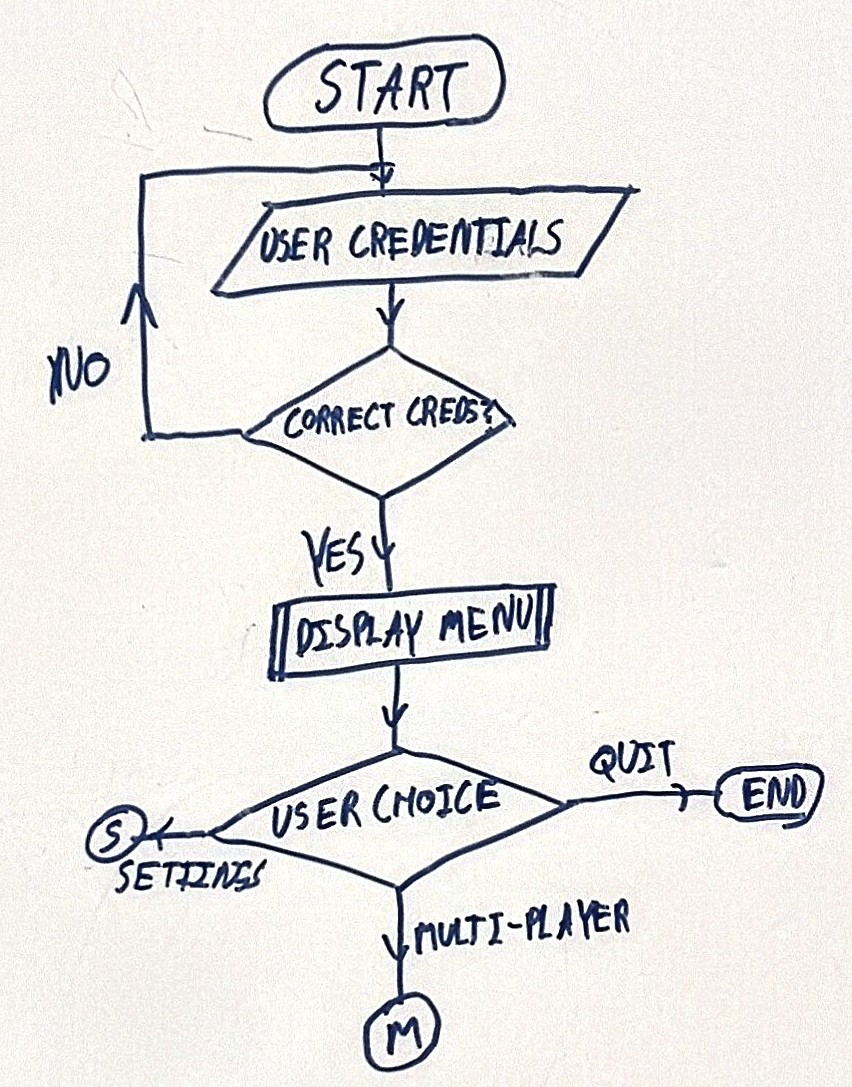
\includegraphics[width=1.0\linewidth]{Analysis/Images/Flowchart_Main.jpg} 
	\caption{Flowchart of main game structure}
	\label{fig:main_game}
	\vspace{-20pt}
\end{wrapfigure}

\vs
Currently, the player's interaction with the game is shown as below. The game will initially take the user's credentials in order to be able to authenticate the user. If the user has entered an invalid username or password, the game will show the original screen again, with a prompt telling them that they have entered the password incorrectly. If the credentials are correct, the user is moved to the main menu level, where they can select to change their settings, to join a multi-player game, or to quite the game. 


\vs
This will then lead to the other modules, which handle each component, and their flow charts are shown as well. This system is very familiar to most people and is quite logical, so there are not many possible misunderstandings. This makes it very effective at communicating to the user what is going on, and so serves its purpose well. Some games have hidden menus when the user clicks on play, such as offering different game modes, but many don't have a way of showing how popular each game mode is. This means that a user may click on a less popular game mode, and wait for a long time before a game lobby is formed.


\vs
There are many actions that a player can undertake, and all of these combined are called the game loop. This forms the basis of the game, and is what people are most interested in. The actions within most FPS games are very similar, such as movement, damage, death / re-spawn, score change, timer change, game end. 

\begin{wrapfigure}{L}{0.38\textwidth}
	\vspace{-20pt}
	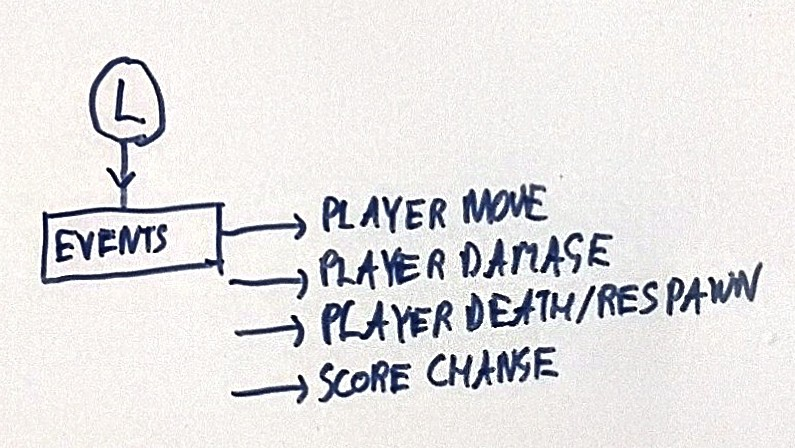
\includegraphics[width=1.0\linewidth]{Analysis/Images/Flowchart_GameLoop.jpg}
	\caption{Flowchart of the game loop}
	\label{fig:game_loop}
	\vspace{-15pt}
\end{wrapfigure}

\vs 
Each client sends a command to the server, indicating the move that has been played, and from that the server can apply those changes and replicate it to all of the other players, ensuring that everyone has a consistent version of the game state. The server is generally placed centrally amongst the players geographically, to ensure that all of them receive roughly equal latency which creates an even playing field. Additionally, once the game has finished, the player is shown an end screen, usually detailing their score, and their performance in the game, and then finally sends them back to the main menu, or gives them the option to play another game.

\vs
\begin{wrapfigure}{R}{0.3\textwidth}
	\vspace{-15pt}
	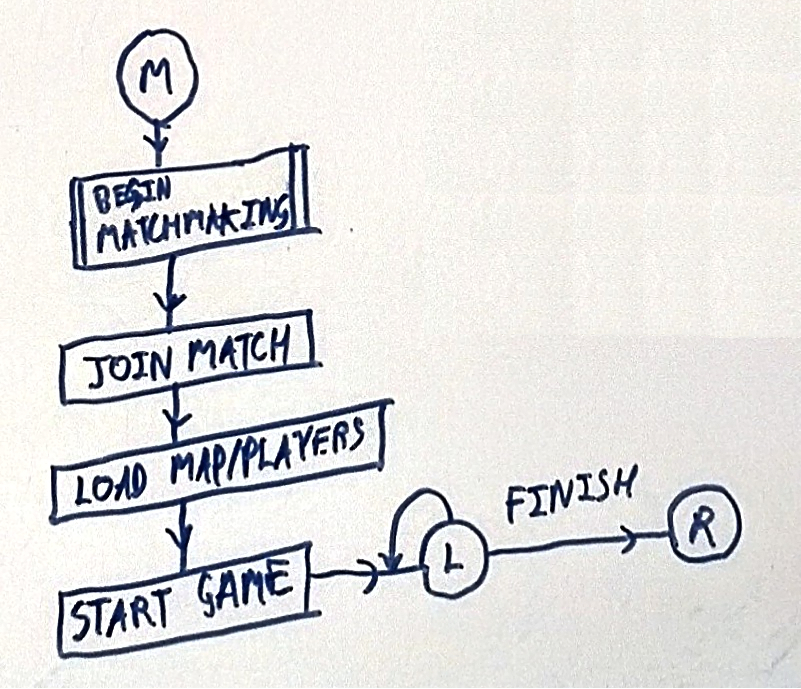
\includegraphics[width=1.0\linewidth]{Analysis/Images/Flowchart_Multiplayer.jpg} 
	\caption{Flowchart of the Multiplayer system}
	\label{fig:multi_flowchart}
\end{wrapfigure}

\vs
Once a user clicks on the multiplayer button, the begin matchmaking procedure occurs. This will allow for a the match to be found which finds a lobby of other players which is usually based on the latency between the player and the server, and any rating system that might be in place. Once this "lobby" is formed, they join a match, and the map and mode of the game is selected randomly. Then, the map is loaded locally on each user's device, and the players are loaded into the map, and the game begins. The game loop as shown above will cycle until one of the game's end conditions are reached, such as a goal limit, or a time limit. 


\vs
Once this happens, any rating changes are applied, and users have the ability to go to the main menu, or play another game. In many cases, the matchmaking procedure can cause long delays whilst players wait for a lobby of their current skill level to form. As a game loses active users, queue times can become much longer as there are just not enough people to fill a lobby, and eventually, people completely stop playing the game. 


\vs
This is obviously not ideal for players who are still interested, and therefore, it is essential that some sort of competitive bots are in place that will allow a player to still get the thrill of playing against people, but not actually require multiple active users to still be online. Additionally, as it is just the player, they can adjust game settings, timings, etc, to their liking, meaning they can find new ways to make the game fun again.

\subsection{Explanation of Choice of Project}

Firstly, a game that can be played on computer provides the best platform for a game, because it is easily accessible to most people, and provides enough computational processing power so that a more detailed game can be run. This however limits my audience to be mainly an audience of PC or laptop users. Additionally, the game will be written in PyGame, which is lightweight and does not require advanced graphics processing.


\vs
Hence, the game is portable, and can be played on a laptop without consuming lots of power. Furthermore, a computational solutions allows for some sort of AI to be implemented, which is almost impossible to do mechanically. This will allow for a much more immersive experience, and encourage people to play without requiring large time commitments. It is also better to run the game on a computer than a mobile device due to the larger computational processing which is possible. It would drain the battery of the user's device if they decided to play on a phone due to the large demands of AI based algorithms, especially neural networks.


\vs
There are multiple platforms to publish games on, such as Steam, and the Epic Games Store, which have very wide audiences, and this adds a sense of community to the game as well as allowing things like leaderboards to form, which will add more of a sense of competition to the game. This can mean that people are more willing to spend more time playing the game. Alternatively, I could create a website that people can access to download the game.

\vs
On top of this, it is generally much clearer to see what is going on when viewed on a larger monitor compared to a mobile device, and this is one of the things that was mentioned by stakeholders as will be shown below. This will also result in a more immersive experience that is more enjoyable for the users.

\vs
Additionally, using a computer will mean that there are more inputs available to the user. For example, from a computer, we have an entire keyboard which provides binary inputs, and a mouse which has further binary inputs in the form of buttons as well as an optical sensor which can provide a much more refined input and a scroll wheel which can be used to allow for quick changes.

\vs
On a phone however, this would be much more limited since any inputs would have to be in the form of touching buttons on the screen, which will take space away from the main content that is display. These buttons need to be clear in their meaning so that it is intuitive how the play the game 

\subsection{Stakeholders}

My stakeholders are generally all people who are too busy to play games during the week. I found these people through online forums, as well as friends who sufferred from similar problems. I sent them a survey to fill which allowed me to gain insight on what things they wanted to get from a game that would encourage them to play during the week. I further asked these people if they would be willing to download test versions of the game and play them and give feedback, which would allow me to consistently improve the game to my stakeholder's needs. The results of the survey are as follows.

\vs
\begin{figure}[H]
    \centering
    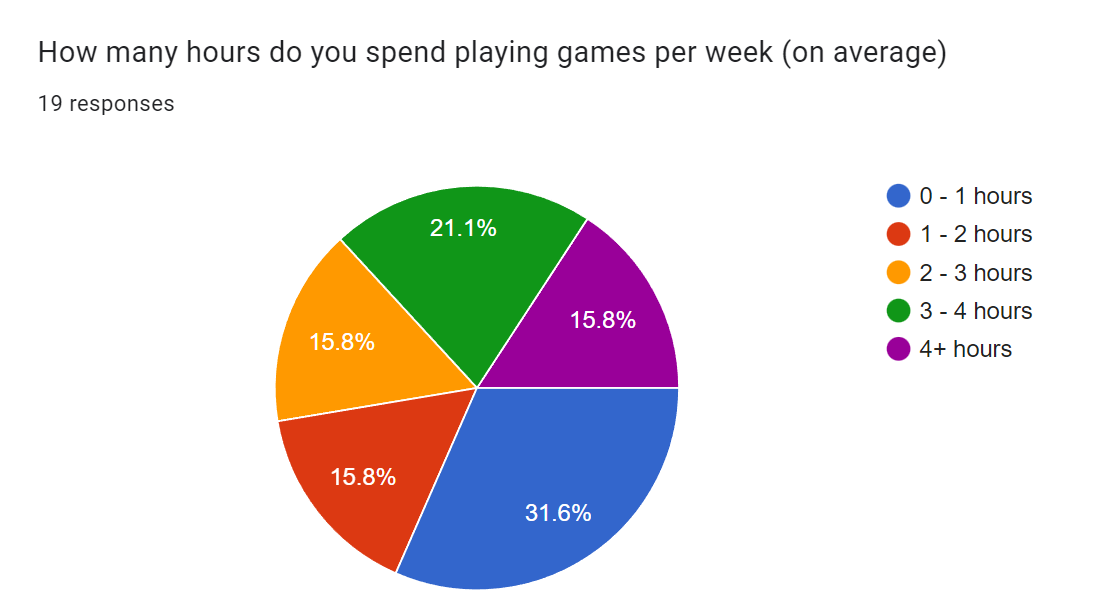
\includegraphics[width=10cm]{Analysis/Images/Analysis_HoursPlayedEachWeek.png}
    \caption{Number of Hours spent playing game per week}
    \label{fig:hours}
\end{figure}

This first question served the purpose of showing me the amounts of time that most people generally spend playing. About a third of people played less than one hour a week, and amongst the other sections, I observed that it was fairly evenly distributed. My game was primarily targeted at the people playing between 0 and 2 hours since this occupies about half of my sample, and is so there is definitely some demand for a game of this type, which focuses on shorter round times to accommodate more games.

\vs
\begin{figure}[H]
    \centering
    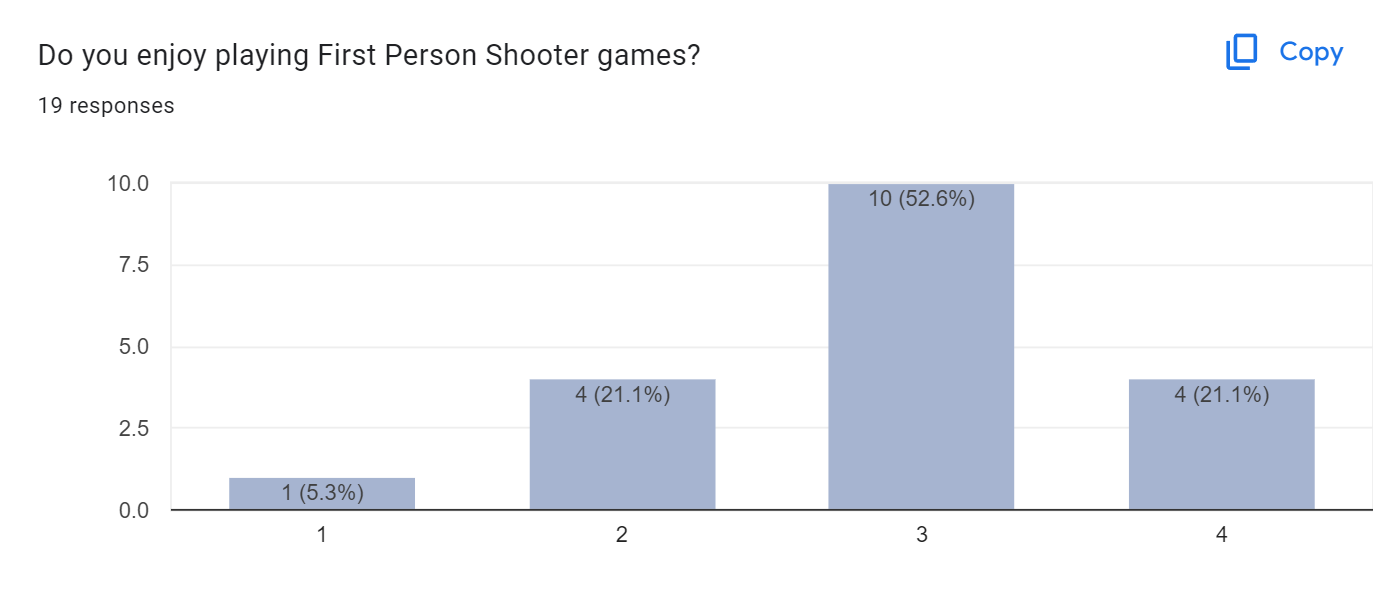
\includegraphics[width=10cm]{Analysis/Images/Analysis_EnjoyFPS.png}
    \caption{Enjoyment of shooter games}
    \label{fig:enjoyment}
\end{figure}

This next question aimed to find the proportion of people which either liked or disliked shooter games. This was important, since I wanted to build a game that people would still be able to enjoy, making them more likely to play in their spare time, or make time out to play it during the week. Additionally, this showed that not everyone likes shooter games, but this is perhaps to be expected.

\vs
\begin{figure}[H]
    \centering
    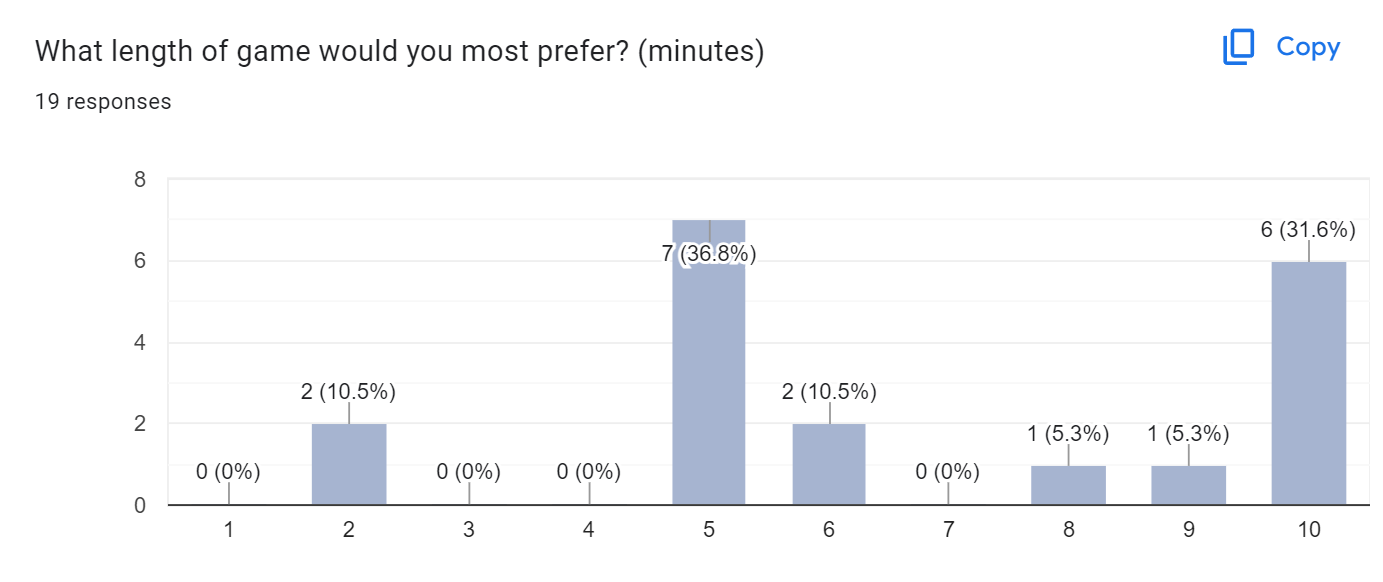
\includegraphics[width=10cm]{Analysis/Images/Analysis_GameLength.png}
    \caption{Desired Game Lengths}
    \label{fig:des_game_length}
\end{figure}

\vs
This showed me roughly how long I should make the rounds in the game. For the most part, the most popular responses were 5 minutes or 10 minutes, but there was some interest in even shorter rounds! In order to resolve this, it may be useful to allow users to set their own time limits in order to allow for variable length rounds, which is tuned to their style. This means that the game adapts to what people want from it, and means that they are more comfortable playing. For example, for some people it may not be possible to play multiple 10 minute rounds, hence they might choose shorter round lengths.

\vs

There were also other questions that were asked, but here is a detailed version of what they revealed. The other results were relating the factors that deterred people from playing during the week. The most common factors were work, school, and a lack of time. Additionally, when asked whether people avoided games with longer round times, 53\% said yes, whilst 47\% said no. The difference was a lot more noticeable however, when asked whether people wanted shorter round times in their games. Here, 58\% said yes, and only 42\% said no. The distribution of round times that people preferred had an average of 6.7 minutes, however, in order to accommodate a strict limit of 3 rounds, we will use 6 minutes instead. This survey provided a useful insight into what people would need to have in a game in order for them to be able to play during their schedules, and made it clear that there is a large audience for this type of game.


\subsection{Interviews}

In order to gain a better understanding of the needs of my stakeholders, I decided to interview them. I asked the following questions and got these responses back. These questions were linked to the questions in the survey but dove into more depth in order to get more information.

\vs
\begin{enumerate}[label=\arabic*)]
    \item Are you comfortable playing games during the week?
    \subitem If not, would you be more comfortable playing a game during the week if you knew that you could control how long you were playing for?
    \item What would be the requirements of a top-down shooter game if you were to play it?
    \item Would you be bothered if you were playing against advanced bots instead of real players?
    \item Would you like to be able to decide the length of your rounds?
    \item Would you like to be able to decide how long you want to play for?
    \item What things would make you more likely to play a game, or make time to play it during the week?
\end{enumerate}

\vs
\subsubsection{Interview 1: Sanjay}
Sanjay, my father, is working a full-time job, and doesn't have much prior experience with playing games. He does, however, play chess occasionally.
\begin{enumerate}[label=\arabic*)]
    \item No. Due to full-time work, I am extremely busy and so don't have the time to play during the evening. Also, having not played many games before, it is slightly daunting.
    \item I should be able to zoom out and find my location on the map, and navigate through it.
    \item I wouldn't be bothered.
    \subitem \textbf{Why not?} I don't want to wait for other players, and bots don't judge you for being bad. You can also choose the expertise of the opponents.
    \item Yes, of course
    \subitem \textbf{Why?} Depending on the time I have, I can setup the game
    \item Yes, a timer system would be nice, to restrict overall play time
    \item Shorter games, quick to setup, and it should be relaxing, not too competitive, and fairly easy to pickup
\end{enumerate}

\vs
\subsubsection{Interview 2: Vaibhav}
Vaibhav is studying robotics and AI at university, and is in a similar position to Moosa - not having much free time during the week. Therefore, he was a suitable stakeholder.
\begin{enumerate}[label=\arabic*)]
    \item No, since I don't have time.
    \subitem \textbf{Follow up:} If I knew exactly what time I would be spending, I would.
    \item Would have to have a great design, many features, many inventory items, like guns, shields, grenades, healables, being able to play with friends and view statistics
    \item No.
    \subitem \textbf{Why not?} Ultimately the game is to play against something. If I still get the dopamine rush, and still enjoy playing, then it doesn't matter. It doesn't present any hindrance. But give the bots random names.
    \item Yes I would like to.
    \item Yes that would be great.
    \item If I didn't have much work helps. Being able to play with friends is nice. Having some kind of ranking system and leaderboard would be great. Getting some sort of currency would be great.
\end{enumerate}

\vs


\subsubsection{Interview 3: Frank}
Frank is a student in my year, and is also very busy. He enjoys playing games, and so he was a viable stakeholder.

\vs
\begin{enumerate}[label=\arabic*)]
    \item Yes, I'd say so.
    \item Mainly good shooting mechanics, but good graphics would also be nice.
    \item Yes
    \subitem \textbf{Why?} Playing against real players is usually much more enjoyable. The bots would have to be very very good otherwise.
    \item Could be nice but probably easiest to switch between long and short games with less rounds at a fixed round length.
    \item Just an enjoyable game with a high difficulty ceiling
    \subitem \textbf{Would you consider a game which has an initially shallow learning curve?} This would make the game too easy and get boring quickly.
    \subitem \textbf{Would you consider a game where the bots get harder the longer you play?} If you can make the hard bots difficult to play against, then that's fine.
    \item A rank system would encourage me to play the game more, since it gives a feeling of achievement.
\end{enumerate}

\vs
\subsubsection{Interview 4: Jay}
Jay is another student in my year, and is also very busy. He enjoys playing games, and so he was a viable stakeholder.

\vs
\begin{enumerate}[label=\arabic*)]
    \item No
    \subitem \textbf{Follow up:} Current amount of stuff I need to do.
    \item I think it has to look nice, and be aesthetically pleasing
    \item That doesn't matter for me
    \item Yes, this sounds nice
    \item Yes, this would be very helpful. Perhaps a timetable so you can't play too early either, and a limit on how late too.
    \item If it involves some interesting mechanics. The week timer system would also be very helpful.
\end{enumerate}

\vs
\subsubsection{Interview 5: Moosa}
Moosa is currently studying engineering at university, and therefore is quite busy and so doesn't have much time to play games during the week.

\vs
\begin{enumerate}[label=\arabic*)]
    \item I don't really play video games anymore, since I don't have much time. I used to play a lot. I do play Minecraft but it is difficult since there aren't that many people to play with either.
    \subitem \textbf{Follow up:} Yeah probably. A social aspect of the game is quite important for me. I don't really play alone, I generally play with friends. If I knew that I could play with a group at a fixed time then definitely.
    \item A compelling story line and if not then multiplayer, different maps, wide range of weapons, different features, interesting mechanics, different game modes, like 1v1 and team matches.
    \item If it was me and my friends against bots that would be fine.
    \item That would be pretty useful. Some games go for quite a long time, so this a useful feature.
    \item This seems like a good feature, and being able to manage time is very helpful. Bad habits and overplaying is quite frequent.
    \item Obviously, popularity of the game helps. In-game interactions are quite funny. The social element of the game is the most important for me.
\end{enumerate}

\subsection{\textcolor{red}{Analysis of Interviews}}

We will look through each question in turn.

\subsubsection{\textcolor{red}{Question 1}}

Most people said that they were not comfortable playing during the week, primarily due to the amount of work that they had to do. This means that short round times, and preferably no queue times would be necessary in order to allow people to feel more comfortable playing games as a way of relaxing during the week.

\subsubsection{\textcolor{red}{Question 2}}

One of the things that was mentioned by users was that the design must be intuitive and easy to use, but also having reliable shooting mechanics that are fun to use. Additionally, almost everyone mentioned that it had to look aesthetically pleasing.

\subsubsection{\textcolor{red}{Question 3}}

Most people were not bothered by the idea of playing against bots instead of real people, although Frank did mention that he would prefer if the bots were good otherwise it would become boring quite quickly. Moosa also mentioned the idea of playing with friends against the bots would be acceptable as well.

\subsubsection{\textcolor{red}{Question 4}}

This was received well, but ultimately, it was not as important, since there was a global timer, but most people preferred having shorter rounds.

\vs
The overall constraint that people wanted was on the amount of time that they spent playing the game. Furthermore, people said that it would be a nice feature to have but not that it had to be in the game for them to play it.

\subsubsection{\textcolor{red}{Question 5}}

Everybody was very accepting of this idea and said that it was something that they would want in the game and would be a useful feature to have. Particularly, having short rounds and then a global timer seemed to be the preferred option.

\vs
This also would help them to solve the problem of having not enough time to play during the week, since now they can limit themselves to only play for a limited amount of time.

\subsubsection{\textcolor{red}{Question 6}}

People mentioned that they would be more likely to play a game during a week if there was some kind of ranking system or a leaderboard of some kind.

\subsection{Stakeholder and Public Requirements Summary}

Here is a list of all of the stakeholder's requirements from my game so far, as well as some things that will improve overall user experience. These were compiled from the interviews, and are justified in the table below.


%\begin{longtable}{|p{4cm}|p{11.5cm}|}
\vs
\begin{center}
\begin{longtable}{|p{4cm}|p{11.5cm}|}
    \hline
     Requirement & Justification\\
    \hline
    \hline
    Shallow Learning Curve & The game must be easy to learn how to play, without requiring a large time investment, which makes the game much more fun to start playing, but must get difficult at some point. This can be enforced by making the mechanics easy to understand and keeping interactions simple.\\
    \hline
    Short queue times & The game must have very short, or no queue times to play, which means that the users can spend more time playing instead of waiting. This was brought up quite frequently in the interviews with stakeholders.\\
    \hline
    Clear UI & The UI must allow the user to understand what each thing represents without too much difficulty. This makes the game more "inviting" to play, and so therefore encourages people to play more.\\
    \hline
    Login System & The project must be able to store user data, such as games played and games won, as well as their login credentials. This will allow them to track their progress and view statistics about their account.\\
    \hline
    Data Security & The project must store this data securely, and allow for logins to be efficient.\\
    \hline
    Leaderboard & The users must be able to view the leaderboard and their position on the leaderboard relative to other players in different categories, such as games played, games won and level.\\
    \hline
    Movement mechanics & There must be a variety of movement mechanics in order to keep the game interesting, and these must be practical to use in game.\\
    \hline
    Time Management & Users must be able to control the amount of time they want to play the game for, and how long the rounds are. Furthermore, players must be able to see how long they have left in a given round.\\
    \hline 
    Gameplay & There must be shooting mechanics, movement, and power-ups that make the game more versatile and interesting to play.\\
    \hline
    Graphics & The game must be visually appealing, or at it should at least be easy to decipher what is going on.\\
    \hline
    Multiplayer & This would allow people to play with friends and would make playing the game more enjoyable and immersive. This is a standard feature of most modern games and would be expected from stakeholders.\\
    \hline
\end{longtable}
\end{center}

These will be taken into account when constructing the design and development of my project.

\subsection{Overall Analysis and Problem Statement}

From all of the analysis done so far and the data collected, we can create a concise summary of it here. This will highlight key points we need to consider, and then we can write a final problem statement, which we can follow.

\vs
Firstly, we saw that the time constraint on people was one of the major restricting factors from them playing games. Having shorter rounds, or allowing people to select the round length would allow them to play games at their convenience, since many games that they may enjoy may have round times that are inconvenient to their schedule and therefore are deterred from playing entirely. The most popular round times were 5 minutes or 10 minutes, so it may well be that I create a system that allows people to select the round time before the round starts. This will be more thoroughly investigated in the Design section of the project. Additionally, I saw that a lot of people enjoyed shooter games, and so this was a safe option for the genre of game, since it would almost certainly guarantee that there is an audience for it.

\vs
Furthermore, I noticed that people didn't enjoy having long queue times since it meant that they would waste a lot of time looking for a game rather than playing. However, this is a universal problem with any multiplayer game, and so it is almost necessarily going to have to be a single-player game, using some sort of algorithm to create an agent that can make "smart" decisions about how to play the game. This will mean that we can add a difficulty setting which will let the player decide which types of bots they would like to play against, making the experience more interactive for the user.

\vs
On top of this, there will be a leaderboard and rank system which be based on the games played and the games won, as well as the score accumulated through playing. This will let the player feel a sense of achievement and this was pointed out by a few of the stakeholders I talked to before. This will be available through the game and users will be able to see where they rank on the leaderboard and how many points they have.

\vs
\textbf{Problem Statement: } The aim of the project is to create a top-down shooter game, named Momentum, which will allow people to play according to their schedules, and let them play against AI bots. The game will allow them to decide how long they want their rounds to be and how long they want to play for overall. They will be able to move their character in different ways, and shoot enemies to increase their score, and the team with the higher score wins.


\subsection{Requirements of the Solution}

The solution must have short queue times, and short round times, ensuring that the player will be active for as long as possible, encouraging them to play further.

\vs
The most common comment on what factors deter people from playing during the week was time commitments, and so it was essential that the game prioritised quick game times, and fast matchmaking, in order to maximise the time that the player is active playing rather than waiting for a game to start.

\vs
In order to solve this, we will use artificial intelligence to create "bots" who can fill lobbies if they are not filled sufficiently quickly. This will allow for games to start as soon as possible, and reduce the amount of time people must wait before a game starts, hence making them more likely to play the game. This promotes starting a game, because the amount of time between pressing the play button and joining a game is shorter, and so people are more inclined to start new games, because they do not take as long to find. Additionally, this will still give the players a feeling of playing with other people, even though they are not.

\vs
Shorter rounds ensure that there is less at stake, and that many rounds can be played in a shorter period of time, and so each game does not feel like as much of a commitment and therefore leaving a game does not have as much of an affect on the player. Additionally, there is no pressure of being judged by other players, or ruining another player's game, since there are just bots playing on the other side, so people will be more likely to judge when they should start and stop playing.

\vs
Additionally, the game will include fast-paced mechanics in order to allow for more intense rounds, which will mean that players see more action in a shorter period of time. There are very very few games which are left in this niche, as many games and franchises, have made their games slower and more tactical. The mechanics within the game will be things just as dashing, sliding, etc. This will allow players to move across the map even faster, and due to the open map design this will be much more easily accomplished. 

\subsubsection{\textcolor{red}{Hardware Requirements}}

In order to run the AI on the machine, the computer must have a CUDA-enabled graphics card. This is quite a steep limitation, but it is available for most people, and so shouldn't be a problem. Furthermore, the computer must have a monitor, keyboard and mouse, because there are the inputs and outputs that are most commonly used and therefore our game will also process using these.

\vs
Additionally, it will need to have at least 4GB of RAM in order to house all of the AI models and all of the data that goes alongside the game. This is necessary, since AI is a key part of our game and we have to load it into memory otherwise the game would be completely unplayable.

\vs
\subsubsection{\textcolor{red}{Software Requirements}}

In order to run the code, the user will need to have CUDA installed, which will allow the neural network to take advantage of the massively parallel architechture of the GPU. This is important as we want to minimise the amount of time it takes to use the model to produce an action. 

\vs

Furthermore, since the game will be written in Python \verb|3.10|, the device must have this version of Python installed, otherwise the game will not operator properly. Additionally, all of the libaries that will be used in the game's final code must be installed also. This is absolutely required, since otherwise the project would take extremely long to complete without libraries, and often libaries have been tested and optimised repeatedly, thus offering a significant performance advantage over raw Python code.

\subsection{Justification of Computational Methods}

The use of computational methods here is paramount. Using a computer will allow us to do multiple things, such as creating an AI which can play with the players. This will require parallel processing in order to achieve smooth gameplay and rendering, as there will be multiple bots which are interacting in the game. Obviously, a reinforcement learning model or similar cannot be done by hand, and so a computer must be used in order to allow for an interactive experience.

\vs
This problem is solvable by computational methods, and is best suited to computational methods, because it is quite difficult to find people to play with in the real world, and they may not be interested, or available to play at that time. By using computers, we can use bots for the person to play against instead of waiting to be connected against other players to play a game. This also the player to dictate the length of the game as well as any game settings they may wish to change. This results in a much more versatile experience for the player and will likely keep them engaged for longer.

\vs
Additionally, we can use computational methods such as abstraction in order to aid the development process. We will examine each in turn.

\vs

\subsubsection{Abstraction}

Abstraction will be used in order to create flowcharts and pseudo-code which will layout the underlying structure of the code. This will allow us to much more easily convert this into the final program, and also mean that we can spot any potential errors before finalising it into code, which will reduce the amount of time we spend debugging our program.

\vs
Furthermore, we will be using external libraries in order to add some abstraction to the graphical and hardware elements of the project. For example, many machine learning libraries are very inefficient to run on a CPU so will use low-level hardware interfaces like CUDA to speed up the process with GPUs which utilise parallelisation in order to do operations like matrix multiplication and addition many times faster. On top of this, a library like PyGame will allow me to focus on the core aspects of the game instead of also having to worry about the implementation of the graphical processing of the game. This adds some abstraction to the game since I no longer have to worry about these things, and it is now hidden by the veil of other classes and methods that have already been tested thoroughly, which means I also can reduce the amount of testing that needs to be done.
\vs

Furthermore, abstraction will be useful as it will allow us to remove details which are irrelevant, and focus on the important attributes and procedures that we need to implement. For example, for a button, we don't need to know what the button does specifically, only that it has a shape, colour, position, and text written on it, and that we want to be able to detect if we are clicking the button at any time.


\subsubsection{Decomposition and Modularity}

Additionally, we will be using classes in the game in order to create a modular program which is much easier to test as we go, and easier to debug. This is useful, since now we can create multiple instances of the same class, such as the player and enemies instead of having to create a number of instances manually. This also allows the game to be more versatile, since we can quickly change singular elements of the game, without having to alter the whole program. This could happen, for example, if users are giving feedback that the game needs changing. It also makes it easier to test and debug, since we can now test each class independently of other classes, and focus on their individual implementations.

\vs
Another way we will be using computational methods is to decompose the problem into smaller, more manageable problems. In this case, we can use the class structure to make the problem much easier to visualise, and code small components of the project. For example, we can work on just the player movement, or the weapons system individually of each other, and then combine them at the end.

\vs

\subsection{Limitations of Proposed Solution}

My main limitation is likely to be hardware. This is in two stages. Firstly, during training, which is done locally on my machine, I will need to use a GPU in order to get a reasonable completion time, as training of AI models can often take hours, or even days. Furthermore, when the player is playing the game, they will be running a model which controls 5 agents, and obviously, this is not an easy computational task, and so it is essential that a GPU is used, and that the game is well-optimised. This can be done using the CUDA library, and the GPU version of PyTorch.

\vs
Additionally, my game will be limited to 2D because I am using PyGame, and so any game that I do make will need to be either top-down or side-on. This means that I will need to use images as my graphics, and potentially use multiple images and cycle through them in order to create the illusion of animation. 

\vs
On top of this, another problem that may potentially arise is that people may not know how to run Python programs, or not have an NVIDIA GPU which is what many modern machine learning libraries run on and is likely what my project will also use. Therefore, it is important to create a list of system requirements for the game that is accessible to most people, and if a GPU is not available the program must be able to run somewhat efficiently on a CPU, which may be challenging. Additionally, packaging the program into an executable file will make it much easier to use for most people, since no specific requirements are needed if it is packaged, except for the platform, but we can package specifically for each platform if needed.


\subsection{Success Criteria}

In order to be able to evaluate the success of my project, I created a list of measurable success criteria that would be able to objectively ensure that the features that were required by the stakeholders would be met.

\vs
These were found using existing computational solutions and the research done by interviewing stakeholders, which we covered before.
\vs


\begin{center}
\begin{longtable}[c]{|p{2.7cm}|p{6.7cm}|p{5.7cm}|}
    \hline
    Name & Success Criterion & Justification\\
    \hline
    \hline
    Gameplay Length & Allow the user to set the total amount of time they would like to play for. & This will let people decide how long they want to play for, and make it so that they can set the game to be as long as is enjoyable for them.\\
    \hline
    Movement & The player can walk around the map, rotate, and cannot pass through other players or objects. & This will make the game more realistic and intuitive to play, since most games already have collisions in them.\\
    \hline
    Player Login & This will let players enter their username and password, which will be checked against the entry in the database. If the login details are correct they will be able to view their profile and play games. & As mentioned before, this will encourage players to play more often, as there is a sense of progress in the game, which makes it more entertaining to play.\\
    \hline
    Rating System & There will be a rating which will be visible to the user and is updated at the end of every match based on the Elo rating system as well as how they performed in the game. & This will further add to a sense of progress, and will provide us with a way to construct leaderboards and things of that nature. Furthermore, it encourages players to get better at the game.\\
    \hline
    Weapon System & The game will contain several different weapons: Assault Rifle, Sniper, and Shotgun. These will each function differently and have different behaviours. & This will add more variety to the game and allow the players to have a better experience.\\
    \hline
    Database System & The database must hold the following information in 3NF.
    \begin{enumerate}
        \item Username, Email, Password
        \item Player Level
        \item Player Experience
        \item Matches Won
        \item Matches Played
        \item Matchmaking Rating (MMR)
    \end{enumerate} & This will allow the user to track their progress, and this will give them a sense of achievement. This encourages the player to play the game more, or make more time to play it during the week.\\
    \hline
    Leaderboard System & There will be a global leaderboard which will show users where they rank in the player-base based on their ranking, and will also show the top 100 or so players of the game. People will be able to search the ratings of other players as well, for example, friends. & This will add a sense of competition into the game and for the players in the top 100 will add an added sense of achievement and further competition to reach rank 1. Furthermore, this will add a bit more of a social element to the game as this will allow people to view what rank their friends are at, and they can compete against each other.\\
    \hline
    Bots & There will be bots which allows for players to play against them even if their friends are not online to play against. These bots must be able to play to a standard such that a human player would not be able to discern between a human and a bot. & This will solve a large part of the problem that people have with currently playing games, namely, a lack of time. Therefore, implementing this feature will allow people to play according to their schedule and convenience, which is a desirable feature as seen in the interviews.\\
    \hline
    Menu System & There will be a menu system that will let a player exit the game, set a timer, and create a game. Within the timer settings, the user can choose how long they wish this timer to be. Within the game creation menu, there will be options for the difficulty of the bots, the length of the rounds and the number of rounds. & This is a useful criterion for success of the project, as many people mentioned that they would be more willing to play if they knew that they would be able to control how long they are playing for, and not play for too long.\\
    \hline
    Difficulty Selection & The player must be able to choose the difficulty of the bots that they are playing against, and playing with. & For players that are less experienced, they can play with better team-mates and worse opponents in order to learn more about the game, and once they are more comfortable can play against better opponents.\\
    \hline
    Game Loop HUD & In the game loop the player must be able to clearly see the team scores, and the time left in the round. & This is important since the player's decision will be guided by the time and score of both teams.\\
    \hline
    Inputs & The user must be able to give inputs using their keyboard and mouse depending on the context. & This is the most commonly available input for a computer or laptop, and therefore, this is the input that our game must be compatible with.\\
    \hline
    Menu Screen UI & The menus must contain clickable buttons which are clearly labelled and will direct the user where they are supposed to. & Buttons are very intuitive to use and will mean that the user can understand what their purpose is when clicking on them. The menu must have buttons, since this is the most common way to interact with a game, and can be easily adapted for other inputs types in the future.\\
    \hline
\end{longtable}
\end{center}

%\clearpage
%Remove bg from flowcharts
%Long table package
%Testing even pretty basic things   
%Include mistakes
%Make mistakes -> J. Savage
%pythonstruct
%show each stage